\chapter{Cosmic Energy Transformations}

%TODO add Heat Death of the Universe to end of this lab.
%TODO:
% - get backup LEDs and flashlights, our own solar panels
% - cart and track worked well
% - double pendulum was too complicated
% - groups with all women could not get the fire syringe to work
% - some syringes leak air and thus don't work

\section{Background: Energy Conservation}

In every closed system, energy is conserved. Mass-energy, that is. Energy is never created or destroyed. This fact has been derived as a mathematical consequence of the fact that the laws of physics do not change over time (the relation between the two is a special case of Noether's theorem, discovered by Emmy Noether, a Jewish-German mathematician described by Einstein as the most important woman in the history of mathematics). Instead of being created or destroyed, energy is transformed from one kind to another.

There are two different kinds of energy, kinetic and potential. Kinetic is energy that something has by virtue of it moving (the faster it is going, the greater the kinetic energy), and potential is stored energy that something has because of its particular position in relation to something else. It is called ``potential'' because it gives the object the potential to do something. There are many different kinds of potential energy, depending on the situation. Examples include gravitational (being further away from massive bodies), chemical (sugar, batteries), electric (electric current), electromagnetic radiation (light, infrared, x-rays), elastic (springs, rubberbands), thermal (warmth), and nuclear (isotopes that can break down or combine to release energy).

We can use the principle of energy conservation to learn about physical processes. For example, if a car is traveling (kinetic energy) and is turned off and slows down and stops, the kinetic energy decreases. That energy did not disappear --- it was either transformed into thermal energy through friction in the brake pads or road, or was stored up again as electrical energy (in the case of regenerative braking in electric vehicles). We even know how much --- the amount of kinetic energy lost is the exact amount of energy gained in these other forms.

%This principle was used to discover neutrinos. In certain radioactive decay, electrons were  particles so unheavy that they were originally thought to have zero mass, and we only know that they have different masses, but not what they are.

%\section{The cosmic Rube Goldberg machine}

\begin{steps}
	\item Since energy is transformed instead of being created or destroyed, start with the kinetic energy of your eyes moving to read this page and trace back the history of energy transformations as far as you can, in as much detail as you can, listing the type of energy in each case. \textbf{Record this for your report.}
\end{steps}

\begin{framed}
Now, you will investigate, quantitatively, several different kinds of energy transformations, qualitatively and quantitatively. You will rotate with other groups around to the different stations as you work, so you might not do the following sections in the order presented.
\end{framed}

Helpful formulas:
\begin{itemize}
	\item Kinetic energy $E_\textrm{k} = \frac{1}{2} m v^2$, where $m$ is mass (in kilograms (kg)) and $v$ is speed of the object (in meters per second (m/s)).
	
	\item Gravitational potential energy for small vertical displacements near the Earth's surface $U_\textrm{grav} = m g h$, where $m$ is mass (in kg), $g$ is the gravitational field strength ($9.8\:\textrm{m}/\textrm{s}^2$), and $h$ is the height above some reference point (in m).
	
	\item The power $P$ (in watts (W)) transferred onto a surface by light is equal to the intensity $I$ (in W/m$^2$) of that light multiplied by the area of the surface $A$ (in m$^2$), or $P = I A$.
	
	\item The power $P$ (in W) transferred in an element of an electric circuit is equal to the current $I$ (in amps (A)) going through the circuit element multiplied by the voltage $V$ (in volts (V)), or $P=IV$.
\end{itemize}

\section{Falling and picking up speed}

There is a track and a toy car that can ride easily on the track.

\begin{steps}
	\item Ensure the track starts and ends at different heights and is fixed in position.
	
	\item Place the car at the top of the ramp and let it go. Notice what energy transformations take place. What types are changing?
	
	\item Measure at least two of the types of energies that are changing, one near the top of the ramp, before the car is released, and one at the bottom of the ramp. You may want to use video tracking to measure speed.
	
	\item Compare the total energy you can measure before and after. Is it the same, within uncertainties? If not, how do you account for the change? Is there an energy type that you are not measuring? What is that energy type? \textbf{Record your calculations and answers.}
	
	\item In what ways is this similar to parts of the process of star formation, and how is it different? You may need to do some research. \textbf{Record your findings.}
\end{steps}

\section{Let there be light! The fire syringe}

Inside the syringe, there is a tiny bit of cotton, surrounded by air at atmospheric pressure. As you push the plunger down, energy is added to the system as you push the air molecules and speed them up. Energy added is equal to $P \:\Delta V$, where $P$ is the pressure of your pushing, and $\Delta V$ is the change in volume. In this system, there are no moving objects to have kinetic energy. If the plunger is pressed quickly, then there is no time for energy to go into heating up the sides of the syringe. Instead, all the added energy heats up the air inside and the cotton itself. If done fast enough, the cotton will ignite.

\begin{steps}
	\item Ensure that there is, in fact, a tiny, wispy bit of unburnt cotton or tissue inside the syringe, and that the piston base is screwed on tightly.
	
	\item Place the syringe on a stable surface and press down on the syringe with great and sudden force. If done properly, you will not damage yourself, and you will see the cotton ignite.

	\item In what ways is this similar to star formation, and how is it different? You may need to do some research. \textbf{Record your findings.}
\end{steps}

\section{Merging black holes --- or are they?}

Two masses each hang from their own $\sim 1\:$meter long string, and the strings are attached to the same overhead point. At rest, they are touching.

\begin{steps}
	\item Move the masses about $10\:$cm apart from each other and push them in opposite directions so that they seem to orbit each other (for example, hold one in each hand the same distance away from you. Then push one away while pulling the other towards you.) Do this until you get a nice smooth, near-circular orbit.
	
	\item As they spin, notice what energy transformations are happening. What kinds of energy is changing, and are each of those types increasing or decreasing? Remember that energy must be conserved, so if one energy type is decreasing, at least one other must be increasing. \textbf{Record your answers.}
	
	\item Now quantify it: measure at least 2 types of energy shortly after you release the masses, and again as they touch each other and become still. Use the formulas above. You may want to use video tracking to measure speed. \textbf{Record your work and results.}
	
	\item Compare the total energy you can measure before and after. Is it the same, within uncertainties? If not, how do you account for the change? Is there an energy type that you are not measuring? What is that energy type? \textbf{Record your calculations and answers.}
	
	\item In what ways is this similar to black holes merging together, and in what ways is this different? You will need to research black hole mergers. \textbf{Record your answers.}
\end{steps}

\section{Absorbing light}

The solar panel is connected to an light emitting diode (LED) that lights up when the panel is exposed to light. A multimeter can be connected to record the current through and voltage across the LED. There is also a light meter that can be used to measure the intensity of incoming light.

\begin{framed}
	In the following steps, if the setup looks correct, but the \textbf{LED is not lighting up}, it might be because the current is going the wrong direction through the LED. Try switching the direction the current goes by switching the cables leading to it.
\end{framed}

\begin{steps}
	\item \textbf{Making the LED light.} Connect the solar panel to the LED as in Fig.\ \ref{et:fig:solar-led} and see that it lights up. Try exposing the solar panel to less and more light and see what happens to the brightness of the LED.

\end{steps}
	
	\begin{figure}
		\centering
		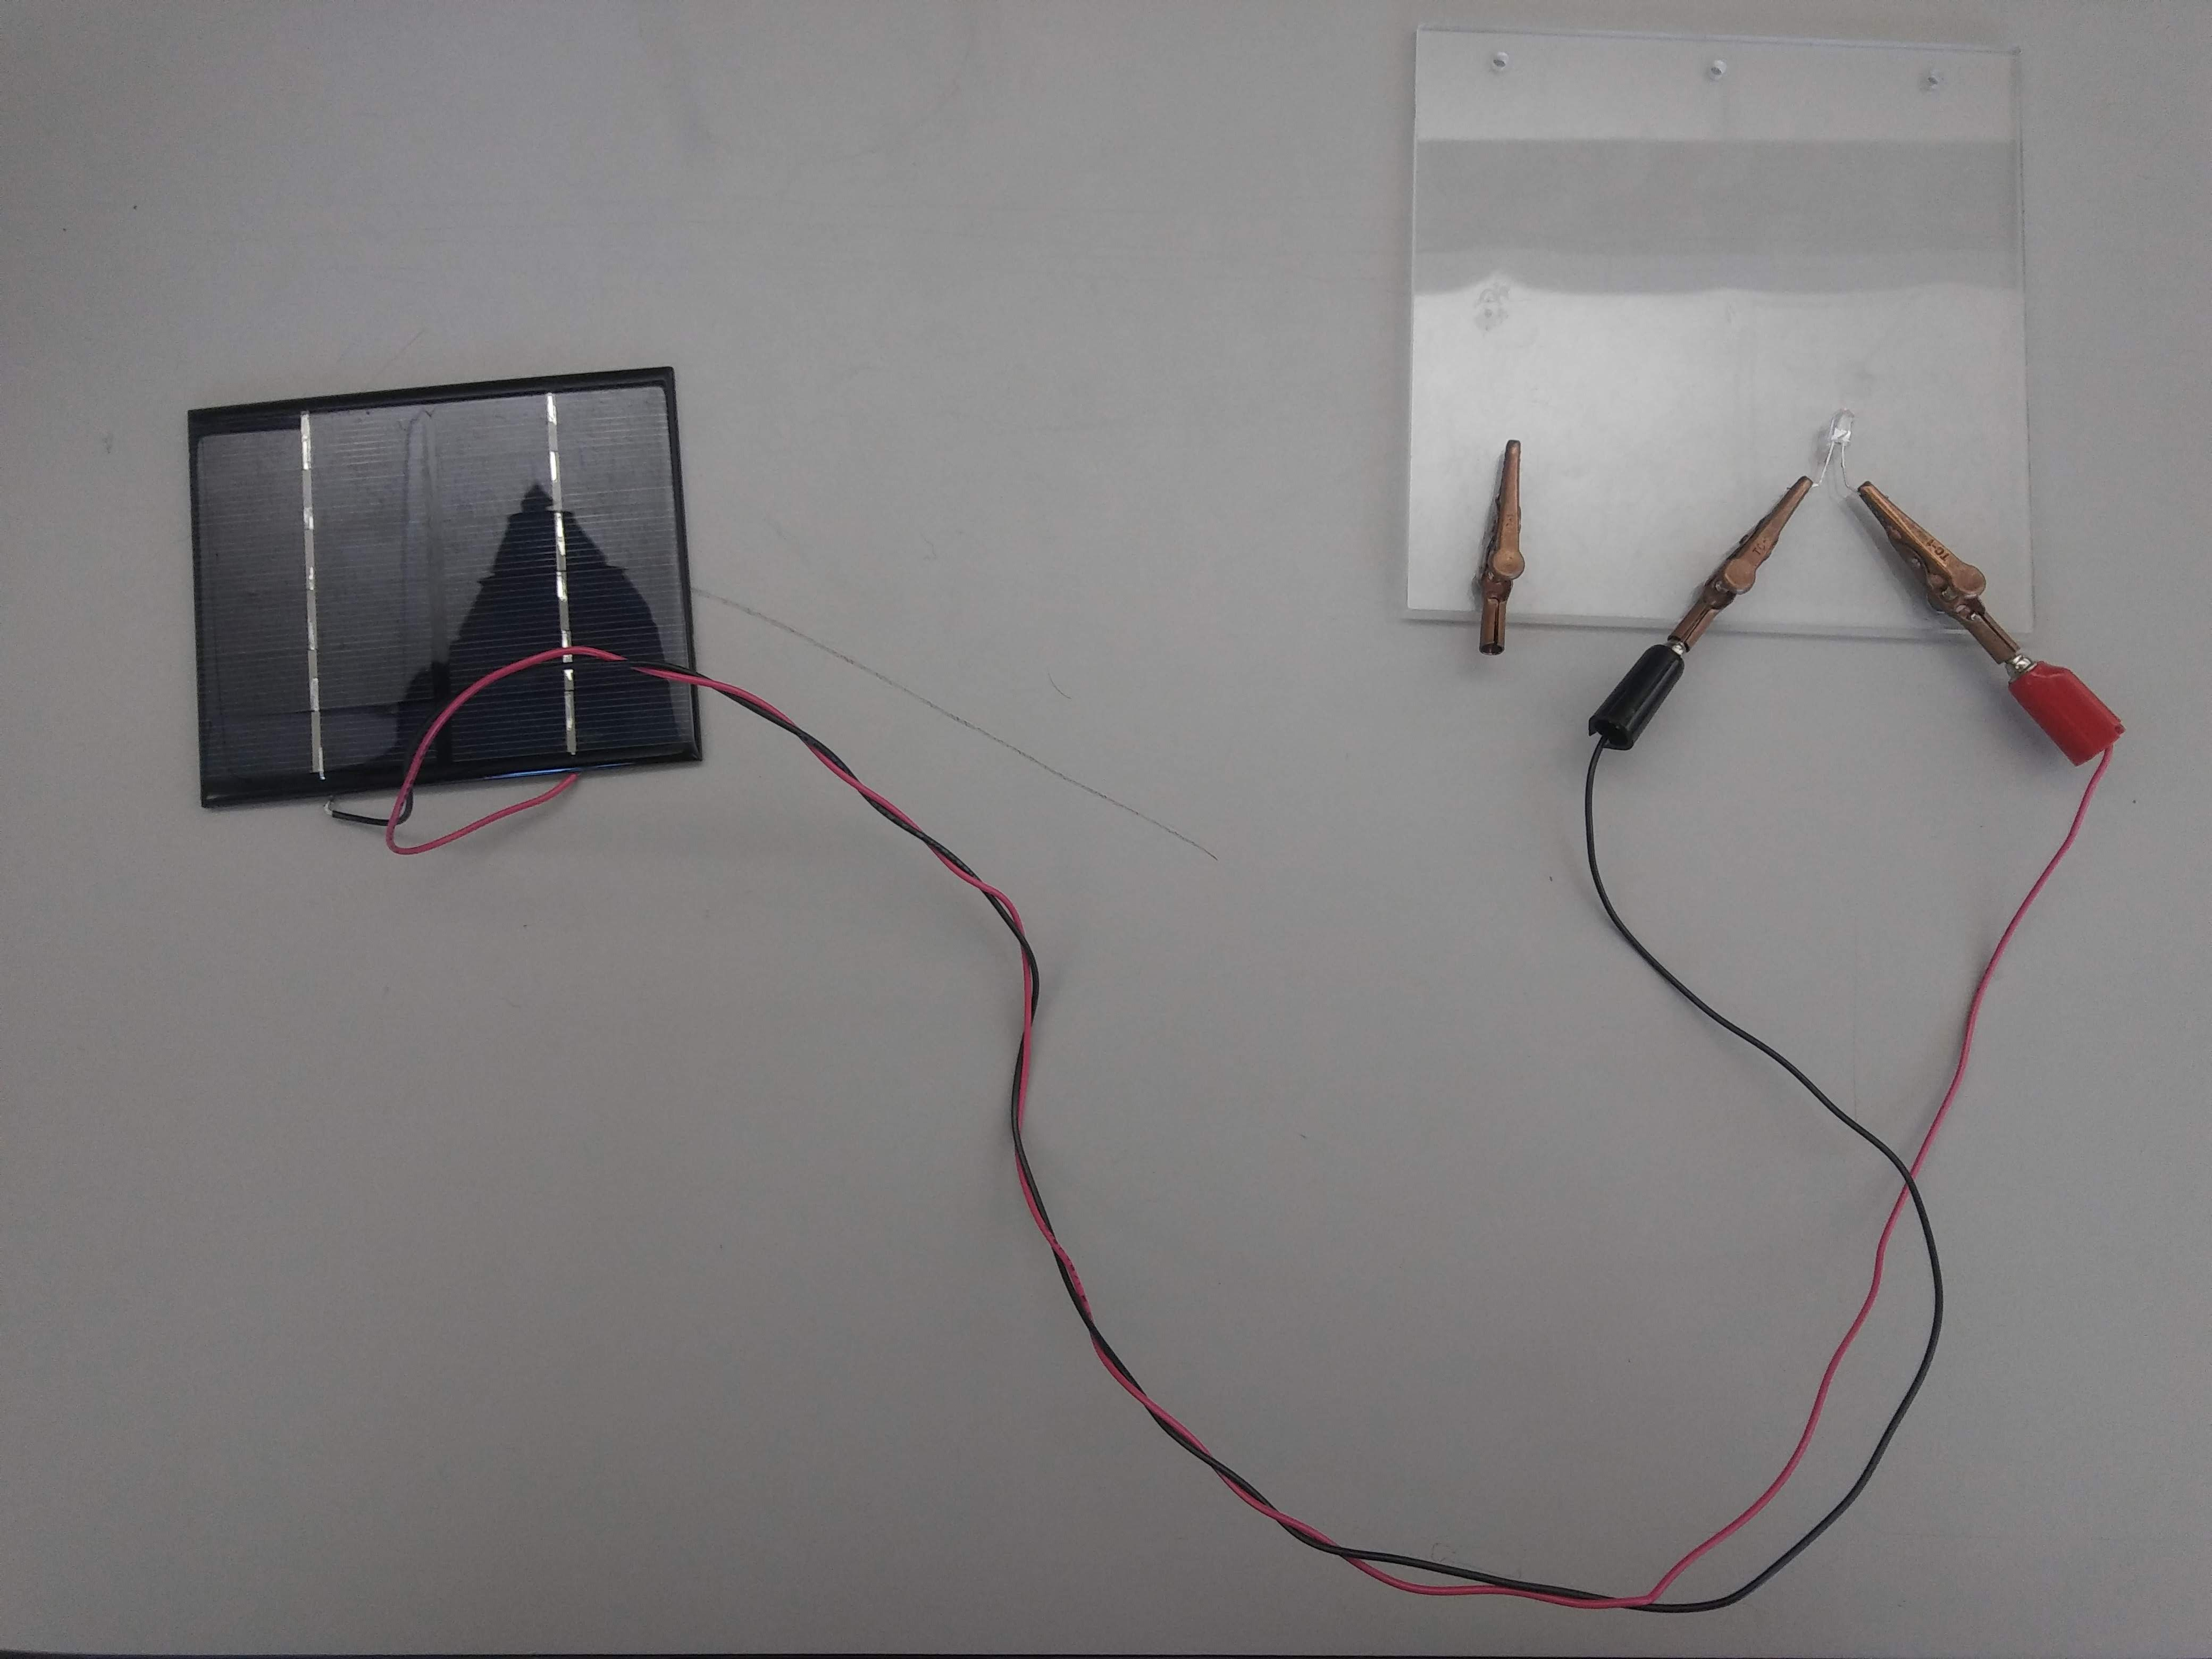
\includegraphics[width=0.7\textwidth]{energy-trans/solar-led}
		\caption{Solar panel connected to the LED.}\label{et:fig:solar-led}
	\end{figure}

Since energy is continuously flowing onto the solar panel and being output from the LED, you will compare the ``power'' instead of the energy. Power is defined as energy per time, so it is how much energy is flowing every second. You can use the last two equations in the Background section to find the input and output power.

\begin{steps}
	\item \textbf{Measure the incoming power.} Turn on the light meter and hold it so that the white dot on top of it is positioned where the solar panel will be. Record the value from the meter. Repeat several times to get an uncertainty.

	\item \textbf{Measure the voltage across the LED.} Ensure that the multimeter is set up to measure voltage (the 'V' setting), one end of the red cable is plugged into the red 'V' socket, and the black cable is plugged into 'COM'. Then plug the other ends of the cables into the two clips attached to the LED. This setup is shown in Fig.\ \ref{et:fig:solar-led-v}. This measures the voltage across the LED, which is like the amount of pressure the solar panel has to apply to get the electrons to go through it.
	
\begin{figure}
	\centering
	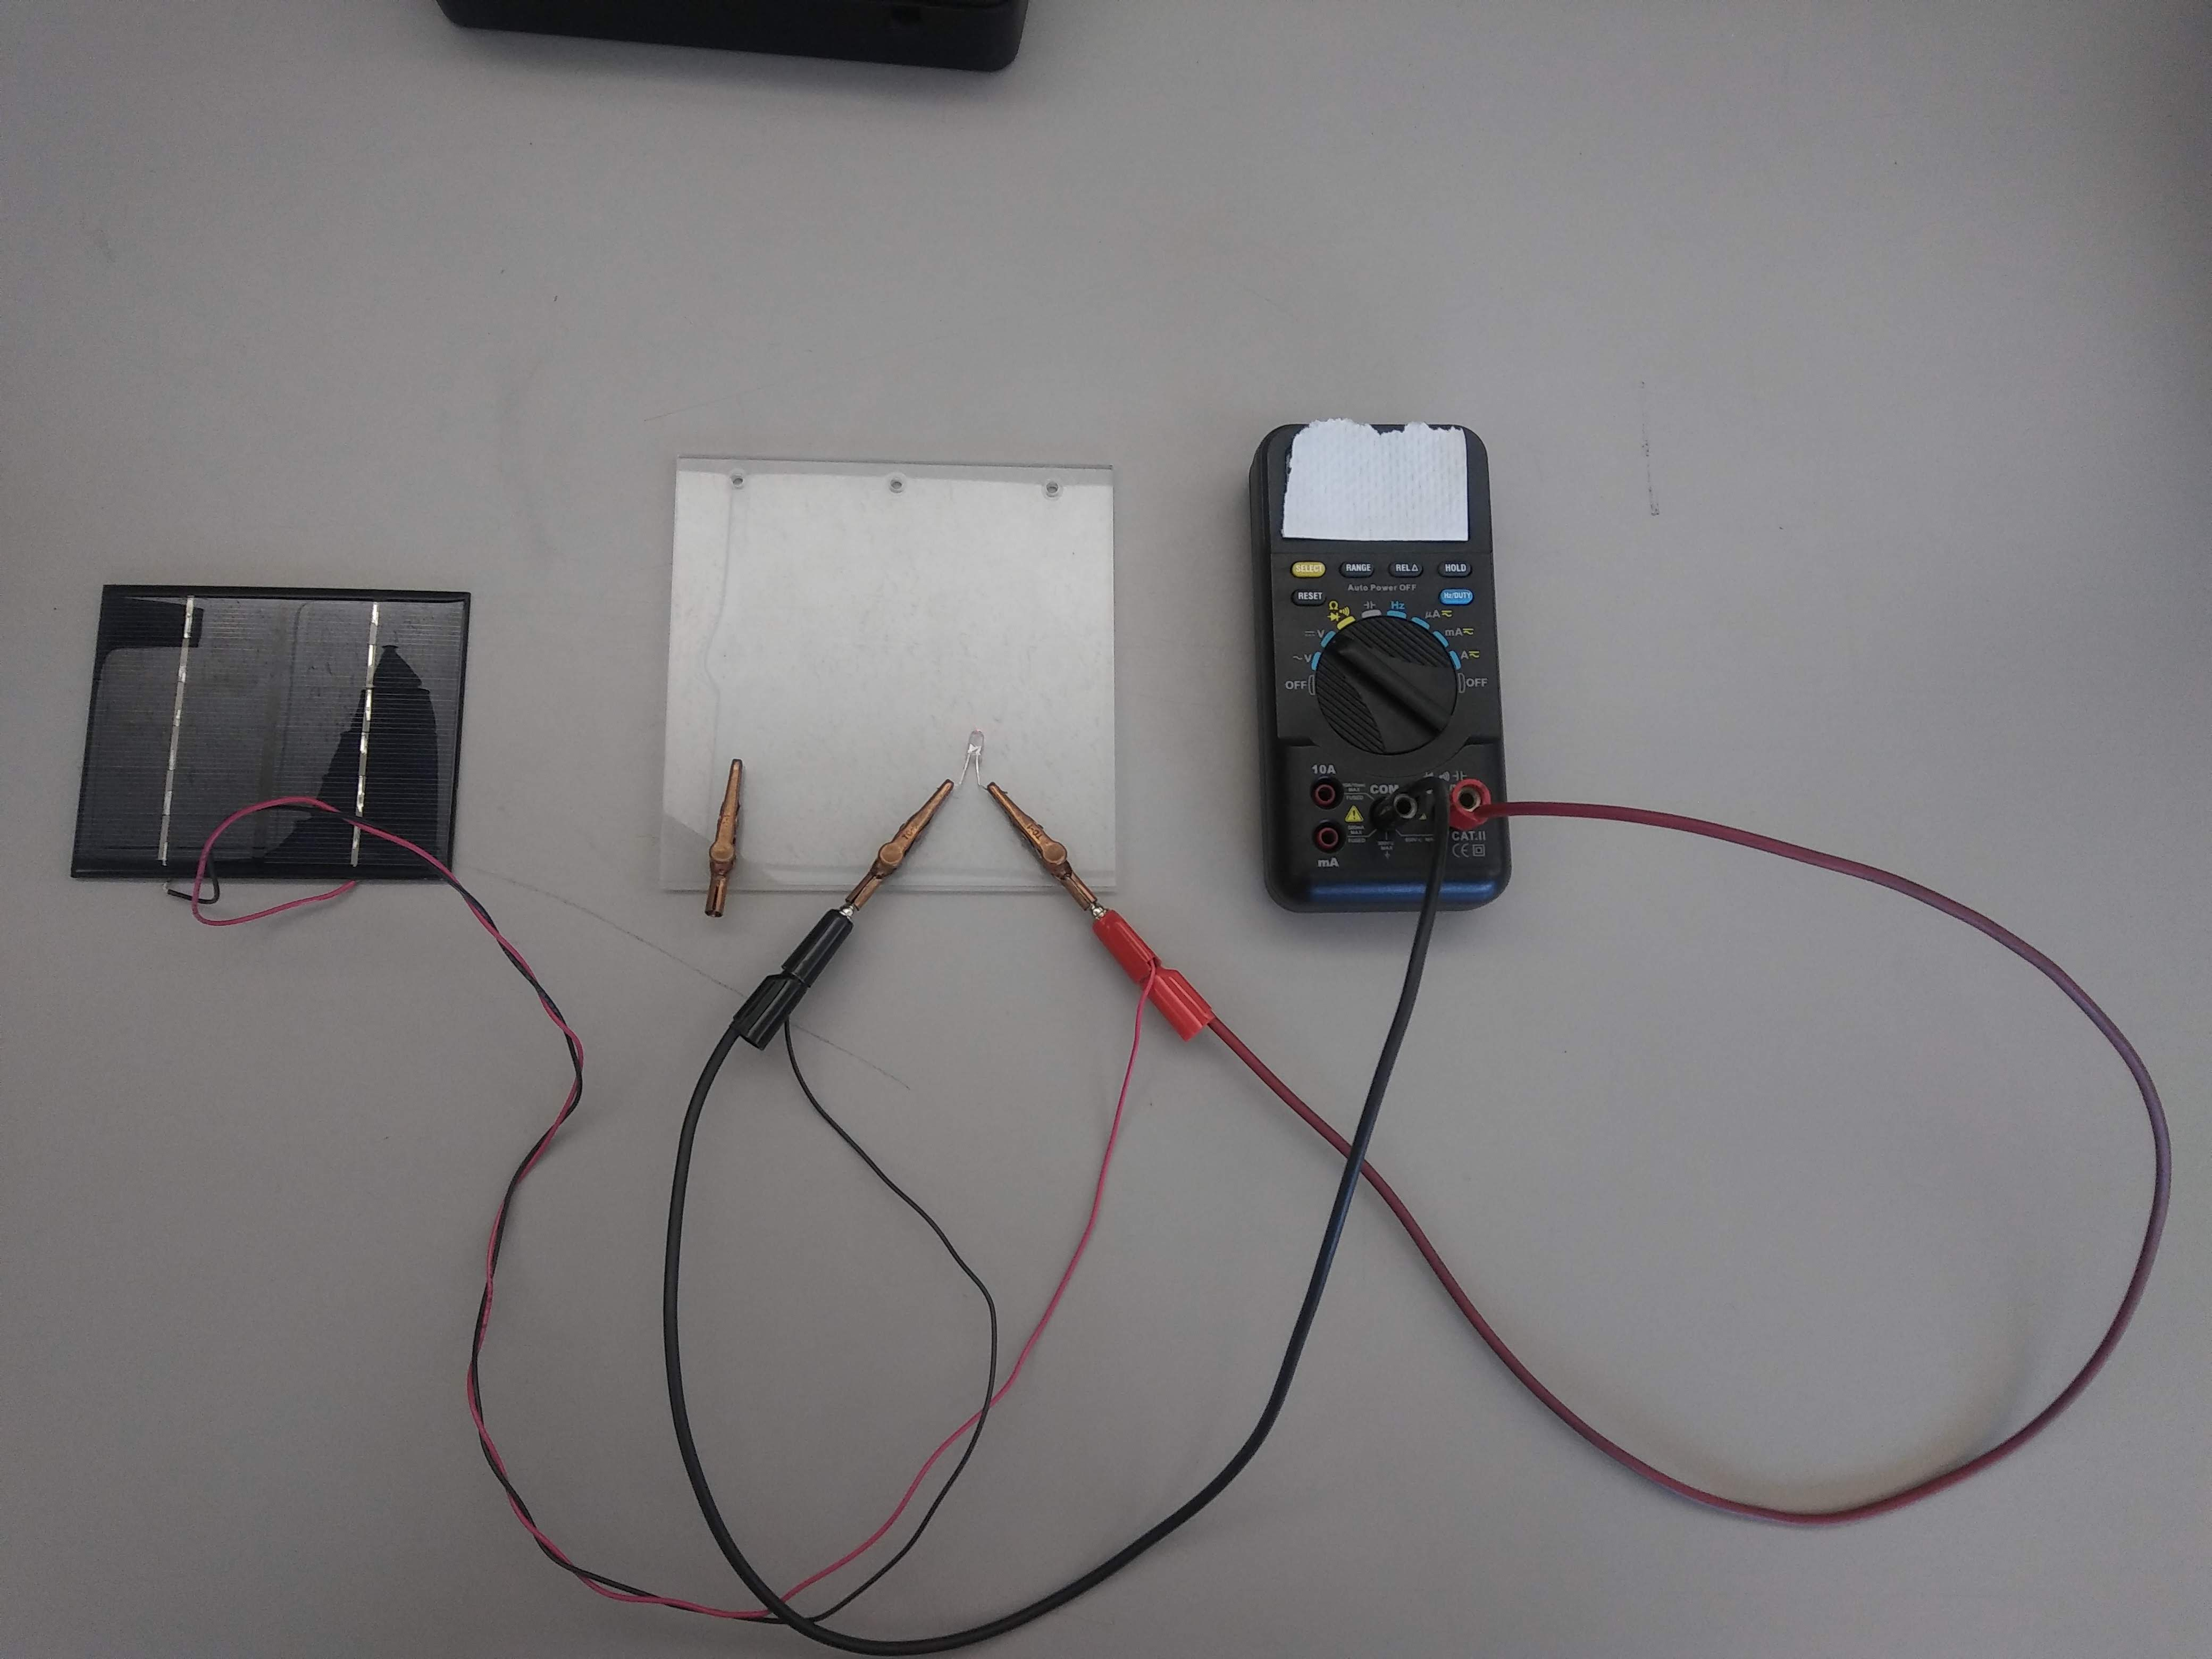
\includegraphics[width=0.7\textwidth]{energy-trans/solar-led-v}
	\caption{Solar panel connected to the LED, with the multimeter attached and set up to measure voltage.}\label{et:fig:solar-led-v}
\end{figure}

	\item \textbf{Measure current through the LED.} Now you will measure the current through the LED. This is a number that is proportional to the number of electrons passing through the wire every second. Ensure that the multimeter is set up to measure current (the `$\mu$A' setting). Then, set up the cables so that the electric current goes from the solar panel's red wire, to the LED, from the other side of the LED to the 'mA' socket on the multimeter, and then from the black 'COM' socket on the multimeter back to the solar panel. This creates a connected loop (circuit) for the electricity to flow through. This setup is described in Figure\ \ref{et:fig:solar-led-ma}. The LED should be lit up when this is correctly set up. \textbf{Record the current reading on the multimeter.}
	
\begin{figure}
	\centering
	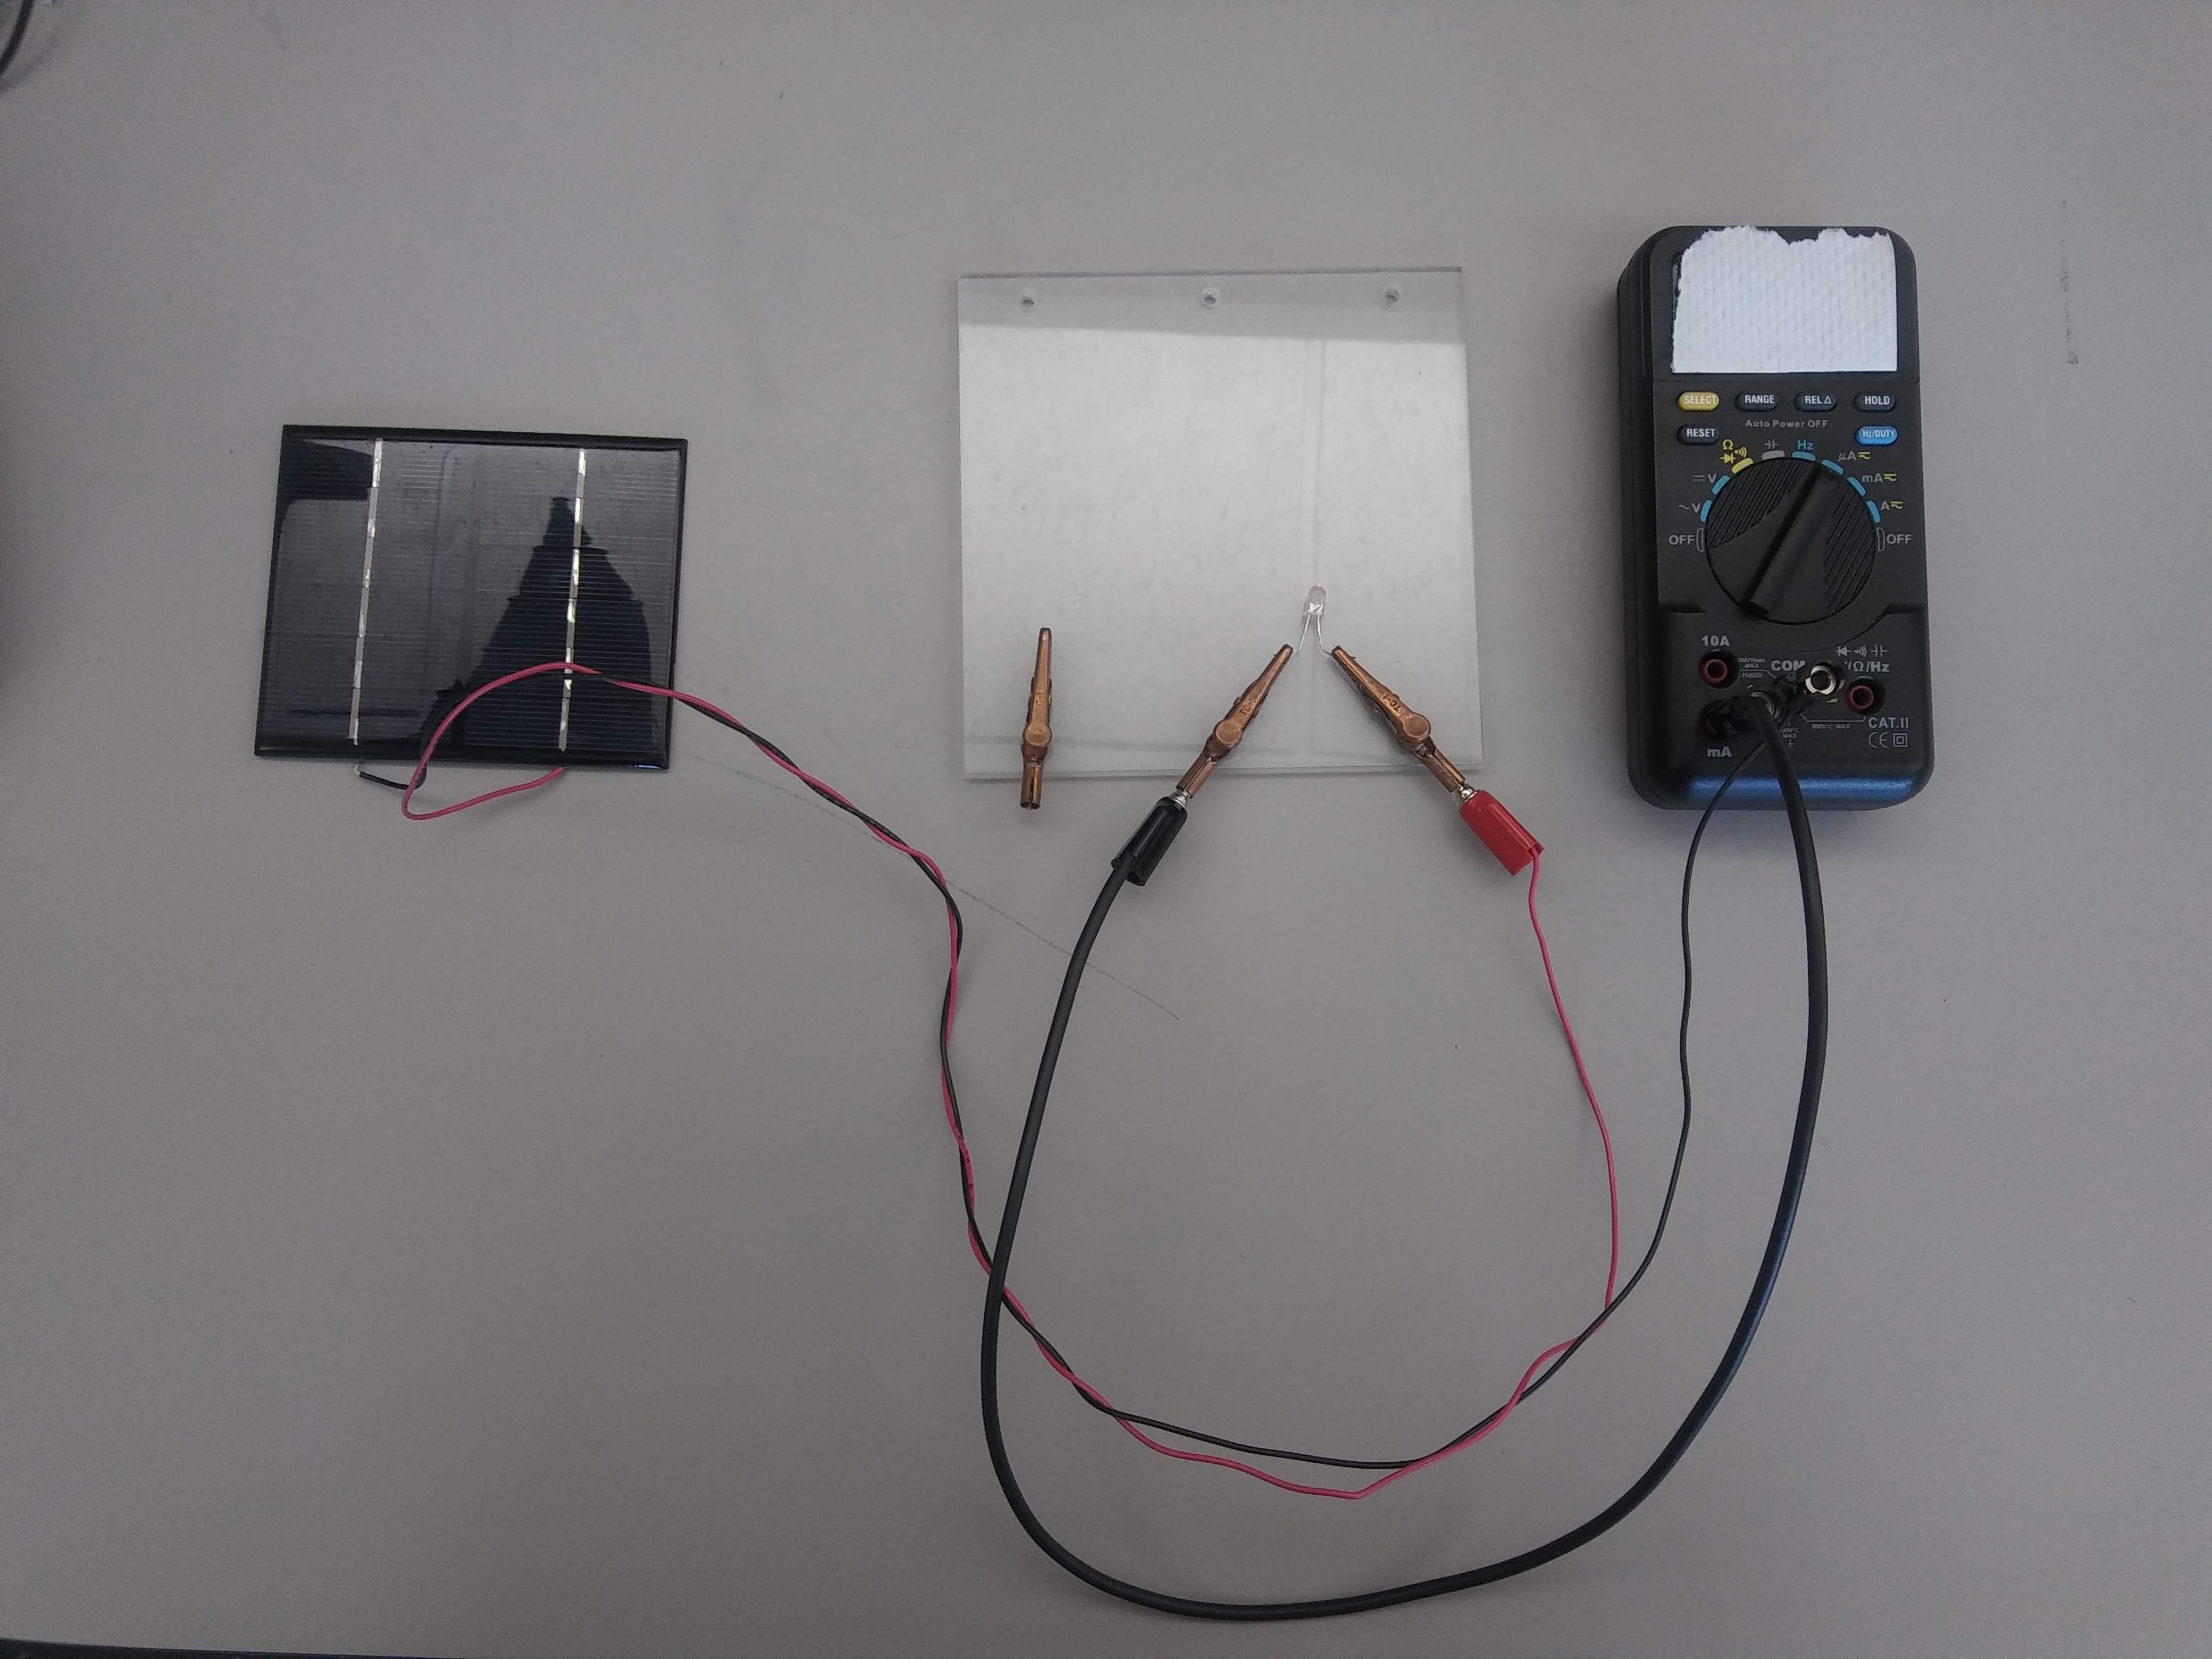
\includegraphics[width=0.7\textwidth]{energy-trans/solar-led-ma}
	\caption{Solar panel connected to the LED, with the multimeter attached and set up to measure current.}\label{et:fig:solar-led-ma}
\end{figure}

	\item Compare the total power input to the solar panel and output through the multimeter. Is it the same, within uncertainties? If not, how do you account for the change? Is there an energy type that you are not measuring? What is that energy type? \textbf{Record your calculations and answers.}
	
	\item In what ways is this similar to light from our sun shining on plants and on water on Earth, and how is it different? \textbf{Record your answers.}
\end{steps}

\section{Report checklist and grading}

Each item below is worth 10 points, and there is an additional 10 points for attendance and participation.

\begin{enumerate}
	\item List of energy transformation history (Step 1).
	
	\item For the car on the ramp: procedure (with sketch of setup), data, analysis, and results including types of energy measured before and after, and amounts of those energies, with uncertainties (Steps 2--4).
	
	\item Car on the ramp: Quantitative comparison of energies before and after, with discussion of extra energy types in play (Step 5).
	
	\item Analogy of car on ramp to star formation (Step 6).
	
	\item Qualitative description of what happened when you pushed down on the fire syringe (Steps 7--8).
	
	\item Analogy of fire syringe to star formation (Step 9).
	
	\item Masses on strings: procedure (with sketch of setup), data, analysis, and results including types of energy measured before and after, and amounts of those energies, with uncertainties (Steps 10--12).
	
	\item Masses on strings: Quantitative comparison of energies before and after, with discussion of extra energy types in play (Step 13).
	
	\item Analogy of masses on strings to black holes merging (Step 14).
	
	\item Data, analysis, and results for the solar panel and LED, including types of energy (per time) measured before and after, and amounts of those energies (per time), with uncertainties (Steps 16--19).
	
	\item Analogy of solar planel to light impinging on Earth (Step 20).
\end{enumerate}